\section{Data Model and ETL}
\label{sec:data}
Given the disparate object models of the data sources that Agent utilizes, it is
necessary to transform data from the original format to a single, source
independent format over which the query executor can operate. This section
defines this target data model and details the ETL process.

\begin{figure}[!h]
\begin{center}
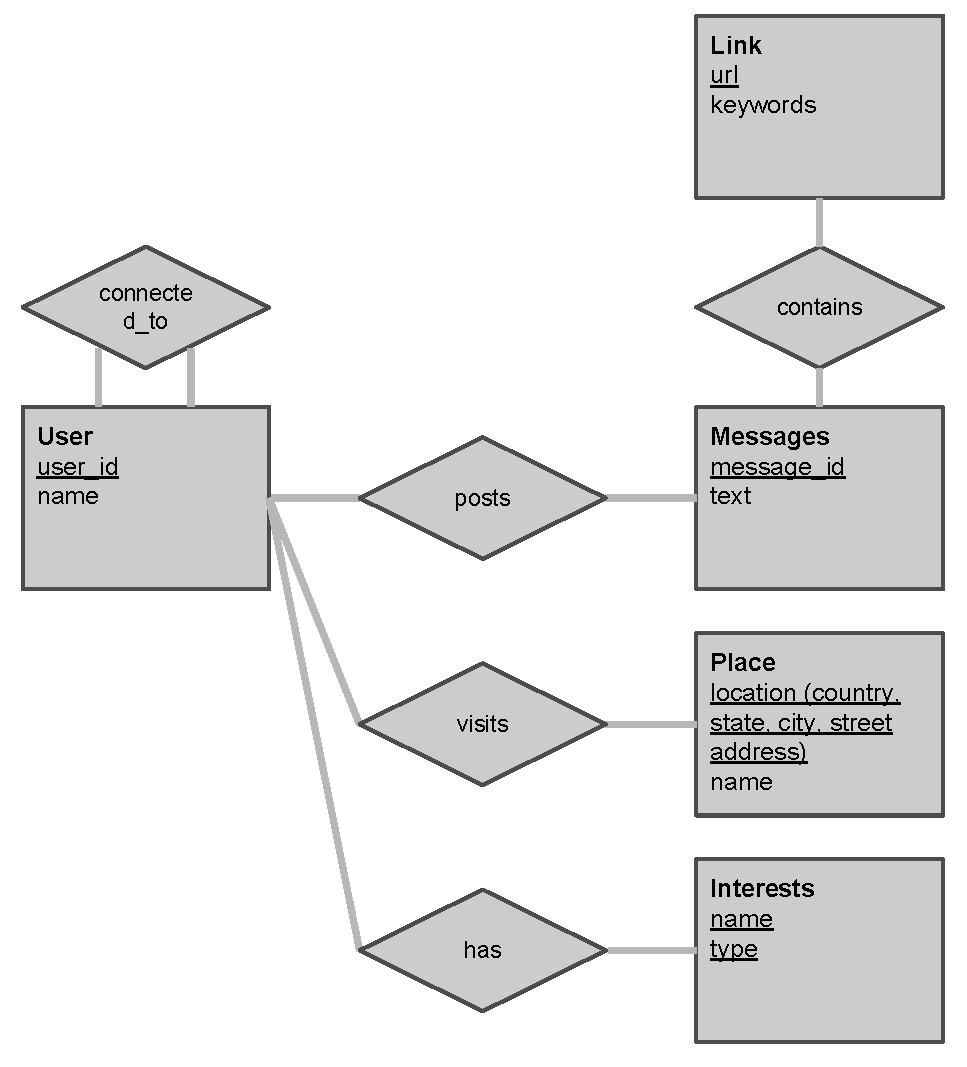
\includegraphics[width=0.5\linewidth]{figs/er-datasource.pdf}
\caption{Entity-Relationship Diagram for Data Sources}
\label{fig:er-datasource}
\end{center}
\end{figure}

We represent social networking data using the Entity Relationship (ER) diagram
shown in Figure~\ref{fig:er-datasource}. Conceptually, we characterize this data
as a set of users and set interactions. Users can be connected among themselves,
and Agent uses those connections to identify candidates for answering a given
query. Interactions are more variable across sites, but on a high level, we
classify them as either posts, profile elements (supplied, structured
information), or locations. The exact mapping of API response objects to these
interaction types varies by site, and furthermore, a single response object
(e.g.\ a Facebook post) might map to multiple interactions (both a post and
location). Agent's backend has a module per data source and performs the mapping
accordingly.

\begin{figure}[!h]
\begin{center}
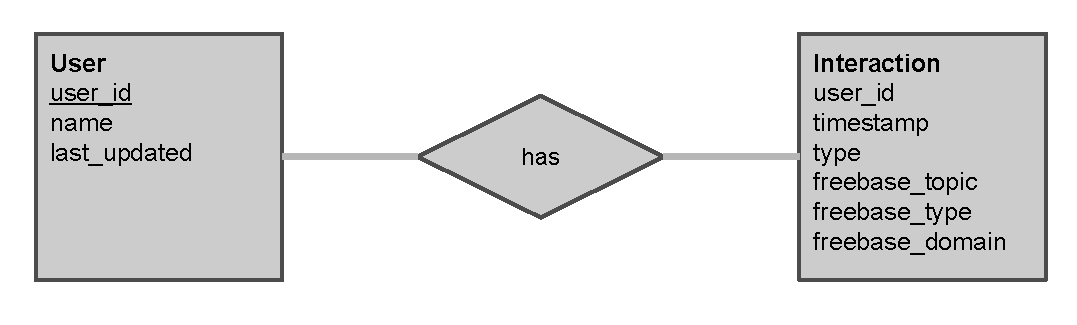
\includegraphics[width=0.5\linewidth]{figs/er-agent.pdf}
\caption{Simplified Entity-Relationship Diagram for Agent Backend}
\label{fig:er-agent}
\end{center}
\end{figure}

Our target data model is shown in Figure~\ref{fig:er-agent}. Note that we have
simplified it for the sake of discussion, representing each of posts, profile
elements, and locations by their superclass, interaction. In practice, we
maintain separate tables for each interaction type, which enables us to more
easily change the information that we store per interaction type as well as to
modify the scoring algorithm.

As shown in the Figure, Agent represents each interaction by the associated
user, a timestamp, and then a collection of Freebase identifiers. Freebase is
``a community-curated database of well-known people, places, and things'' that
represents its entities as nodes in a graph connected to each other by various
properties \cite{freebase, freebase-api}. Most importantly, Freebase taxonomizes
each entity by a domain and a type (actually a set of them), which allows users
to classify topics by knowledge area, a perfect fit for our application.

Although our current implementation of Agent uses Freebase identifiers, Agent is
not dependent on Freebase. Agent could very easily use Wikipedia or
other identifiers or even a custom knowledge representation format. However,
Freebase is particularly convenient and well-supported and therefore a good
choice for use in our application.

Given the data models described above, the ETL process is straightforward. Given
an API response, the data module generates a set of {\it user\_id, timestamp,
interaction\_type, entity} tuples. The entities are extracted from the original
response object based on the objects format. For example, profile elements are
usually limited to entities recognized by the social networking site, so the
entity mapping is simply the API response. On the other hand, a post generally
contains a string of text, so the data module performs term extraction
similarly to the query parser (see Section~\ref{sec:query-parser}).

After generating the intermediate tuples, the data module takes those tuples and
generates a final set of tuples with the attributes shown in
Figure~\ref{fig:er-agent}. Specifically, given an entity, the data module uses
the Freebase search API to generate a candidate list of Freebase topics, and
then selects the most likely topic. It then retrieves that topic's type (or in
the event that the topic falls under multiple types, the most notable one) and
similarly its domain. This data is then combined with the other input and stored
as a tuple in the appropriate table in the database, based on the interaction
type.

